\documentclass{article}
\usepackage[utf8]{inputenc}
\usepackage{graphicx}

\title{Reporte Técnico}
\author{Diego Iván Perez Conde}
\date{March 2021}

\begin{document}

\maketitle

\section{Introduction}

\text{El trabajo que llevare a cabo es una red neuronal que estara echa sobre matlab pero antes de llevar a cabo este proceso hay que empezar con varias definiciones acerca de mi tema, definiremos que es una red neuronal artificial y su objetivo.
Las redes neuronales artificiales (tambien conocidas como sistemas conexionistas) son un modelo computacional el que fue evolucionando a partir de diversas aportaciones cientıficas que estan registradas en la historia. 
Consiste en un conjunto de unidades, llamadas neuronas artificiales, conectadas entre si para transmitirse señales. La información de entrada atraviesa la red neuronal (donde se somete a diversas operaciones) produciendo unos valores de salida.

El objetivo de la red neuronal es resolver los problemas de la misma manera que el cerebro humano, aunque las redes neuronales son más abstractas. Las redes neuronales actuales suelen contener desde unos miles a unos pocos millones de unidades neuronales.
 }
 
\textbf{¿Cómo funcionan las redes neuronales?}

\text{Una red neuronal combina diversas capas de procesamiento y utiliza elementos simples que operan en paralelo, y están inspiradas en los sistemas nerviosos biológicos. Consta de una capa de entrada, una o varias capas ocultas y una capa de salida. Las capas están interconectadas mediante nodos, o neuronas; cada capa utiliza la salida de la capa anterior como entrada.}


\section{Desarrollo}

\text{Para esto el desarrollo de mi tema sera llevado a cabo sobre matlab y sera llevar a cabo figuras o dibujos ya sea de personajes de videojuegos o solo imagenes que son llevadas a cabo en pixel art, para el desarrollo del tema.Para eso cree matrices de 16x16 ya que mis figuras podueden muy bien quedar en ese tamaño de la matriz, para esto mi red neuronal necesita saber cuantas figuras va poder ser reconocida por la red neuronal, para eso tomamos el numero de datos de nuesta matriz y esta la multiplicamos en este caso seria: 16x16=256 y nuestro resultado que hayamos obtenido sera multiplicado por 0.15 quedando: 256x0.15=38.4 con esto sabria cuantas figuras debera reconocer mi red neuronal que despues debera ser implentado el desarrollo en C++.}\\

\text{Bueno con la informacion obtenida ahora debo poder llevar a cabo el entrenamiento de mi red neuronal, con lo que usare octave que esta basado en matlab, entonces para poder representar mis patrones a identificar de la matriz uso mi matriz de 16x16 y bueno para identificar el simbolo o figura uso el numero uno (1) para marcar el contorno de mi figura en este caso, entonces el (0) es como mi espacio en blanco pero en este caso como estamos entrenando la red neuronal sobre matlab esta pasara los numeros (0) a (-1) para poder identficarlo en el lenguaje del mismo, con ello una vez finalizo, pasamos a nuestro IDE donde se creara el codigo en c++ para nuestra red neuronal en este caso la representaremos con los valores 0 y 1 como se habia dicho anteriormente se puede observar asi.}


\begin{figure}[htb]
\centering
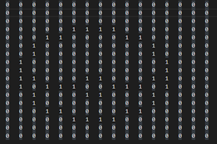
\includegraphics[width=0.3\textwidth]{Imagen1.png}
\caption{Patron de entrada}
\label{fig:tigre}
\end{figure}
\text{Este es el patron de nuestra entrada con el cual si fue reconocido mostrara la salida}

\begin{figure}[htb]
\centering
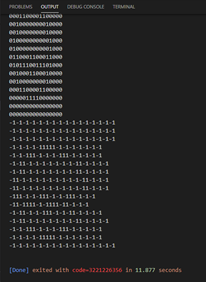
\includegraphics[width=0.3\textwidth]{Imagen2.png}
\caption{Patron de salida}
\label{fig:tigre}
\end{figure}
\text{Esta es la salida de nuestra entrada con la cual podemos decir que si quedo muy bien ejecutada}


\section{Conclusión}
\text{Para finalizar nuestro pequeño analisis o reporte podemos decir que las rede neuronales son un gran apoyo para todo lo que queramos llegar hacer con ellas ya que son muy utiles y eficazes.
Con base a lo que vimos este es un ejemplo basico de como funciona una red neuronal.}



\end{document}
